\documentclass[dvipsnames,tikz]{standalone}
\usepackage{amsmath}
\usepackage{xcolor}
\usepackage{tikz}
\usetikzlibrary{calc}
\usetikzlibrary{decorations.pathreplacing,calligraphy,3d}
\usetikzlibrary{positioning}

% Generation using https://opendsa-server.cs.vt.edu/embed/PrimPE

\begin{document}
	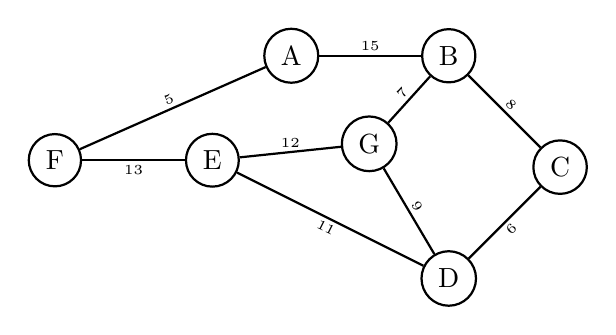
\begin{tikzpicture}[node distance={20mm}, thick,main/.style = {draw, circle}] 
		\node[main] (A) {A}; 
		\node[main] (B) [right of = A] {B};
		\node[main] (C) [below right of = B] {C};
		\node[main] (D) [below left of = C] {D};
		\node[main] (E) [above left = 1cm and 2.5cm of D] {E};
		\node[main] (F) [left of=E] {F};
		\node[main] (G) [above left = 1.2cm and 0.5cm of D] {G};
		
		\begin{scope}[font=\tiny, inner sep=0.5mm]
			\draw (F) -- node[midway, above, sloped] {5} (A);
			\draw (C) -- node[midway, below, sloped] {6} (D);
			\draw (G) -- node[midway, above, sloped] {7} (B);
			\draw (B) -- node[midway, above, sloped] {8} (C);
			\draw (D) -- node[midway, above, sloped] {9} (G);
			\draw (D) -- node[midway, below, sloped] {11} (E);
			\draw (E) -- node[midway, above] {12} (G);
			\draw (E) -- node[midway, below] {13} (F);
			\draw (A) -- node[midway, above] {15} (B);
		\end{scope}
	\end{tikzpicture} 
	
	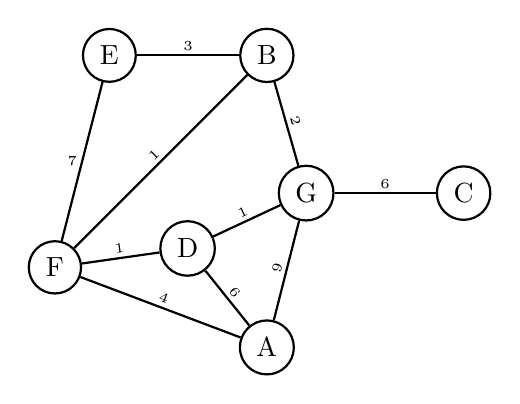
\begin{tikzpicture}[node distance={20mm}, thick,main/.style = {draw, circle}] 
		\node[main] (A) {A}; 
		\node[main] (B) [above = 3cm of A] {B};
		\node[main] (C) [below right = 1.25cm and 2cm of B] {C};
		\node[main] (D) [above left = 0.75cm and 0.5cm of A] {D};
		\node[main] (E) [left of = B] {E};
		\node[main] (F) [below left = 2.2cm and 0.2cm of E] {F};
		\node[main] (G) [left of = C] {G};
		
		\begin{scope}[font=\tiny, inner sep=0.5mm]
			\draw (A) -- node[midway, above, sloped] {6} (D);
			\draw (D) -- node[midway, above, sloped] {1} (F);
			\draw (F) -- node[midway, left] {7} (E);
			\draw (E) -- node[midway, above] {3} (B);
			\draw (B) -- node[midway, above, sloped] {2} (G);
			\draw (B) -- node[midway, above, sloped] {1} (F);
			\draw (G) -- node[midway, above] {6} (C);
			\draw (A) -- node[midway, above, sloped] {9} (G);
			\draw (D) -- node[midway, above, sloped] {1} (G);
			\draw (A) -- node[midway, above, sloped] {4} (F);
		\end{scope}
	\end{tikzpicture} 
\end{document}